\cleardoublepage
\newpage
\ifdefined\EnableIncludeImages
    \ThisULCornerWallPaper{1.0}{chapterimage.eps}
\fi
\chapter{Zandor}
Después de la muerte de Zorra, toda la familia se quedó muy triste, pues a pesar de sus malas costumbres, ella siempre fue muy amorosa con todos nosotros, por eso sentíamos su falta como si fuese un miembro de la familia.
Así, pasamos mucho tiempo llorando, sobretodo mis hermanas y yo, que aún eramos niños.
Muchas veces vi a Teodosia --- mi hermana mayor, la cual cariñosamente llamábamos ``Tulaco'' ---, iniciar a llorar en silencio al ver el lugar donde Zorra dormía; inclusive Diofelia --- ``Dio'', mi hermana menor ---, a pesar de su corta edad, yá sabía distinguir la muerte y la ausencia que esta deja.
Yo también lloraba, tal vez más que ellas, porque Zorra era mi compañera fiel, ella me seguía a todos los lugares donde yo iba; pues, al ser el hijo hombre de la casa, yo era el que tenía que salir a trabajar en la chacra con mi papá, y Zorra siempre hacía mas alegres y memorables esos momentos.
Nuestro único consuelo era que teníamos a Zandor; nosotros lo amábamos por ser el último regalo que Zorra nos dejó.
Yo miraba a Zandor, todo pequeño y negrito y pensaba que era muy lindo. Su presencia me decía que de alguna forma, una parte de Zorra aún estaba con nosotros.
Así, Zandor creció siendo criado con mucho cuidado y cariño por todos nosotros;
entretanto, la personalidad de Zandor era distinta de la personalidad de su mamá, él era un perro muy honrado y era evidente para nosotros que el no tenia ninguna de las malas costumbres de Zorra.
\ifdefined\EnableIncludeImages
\begin{wrapfigure}{r}{0.45\textwidth}
  \begin{center}
  \vspace{-20pt}
    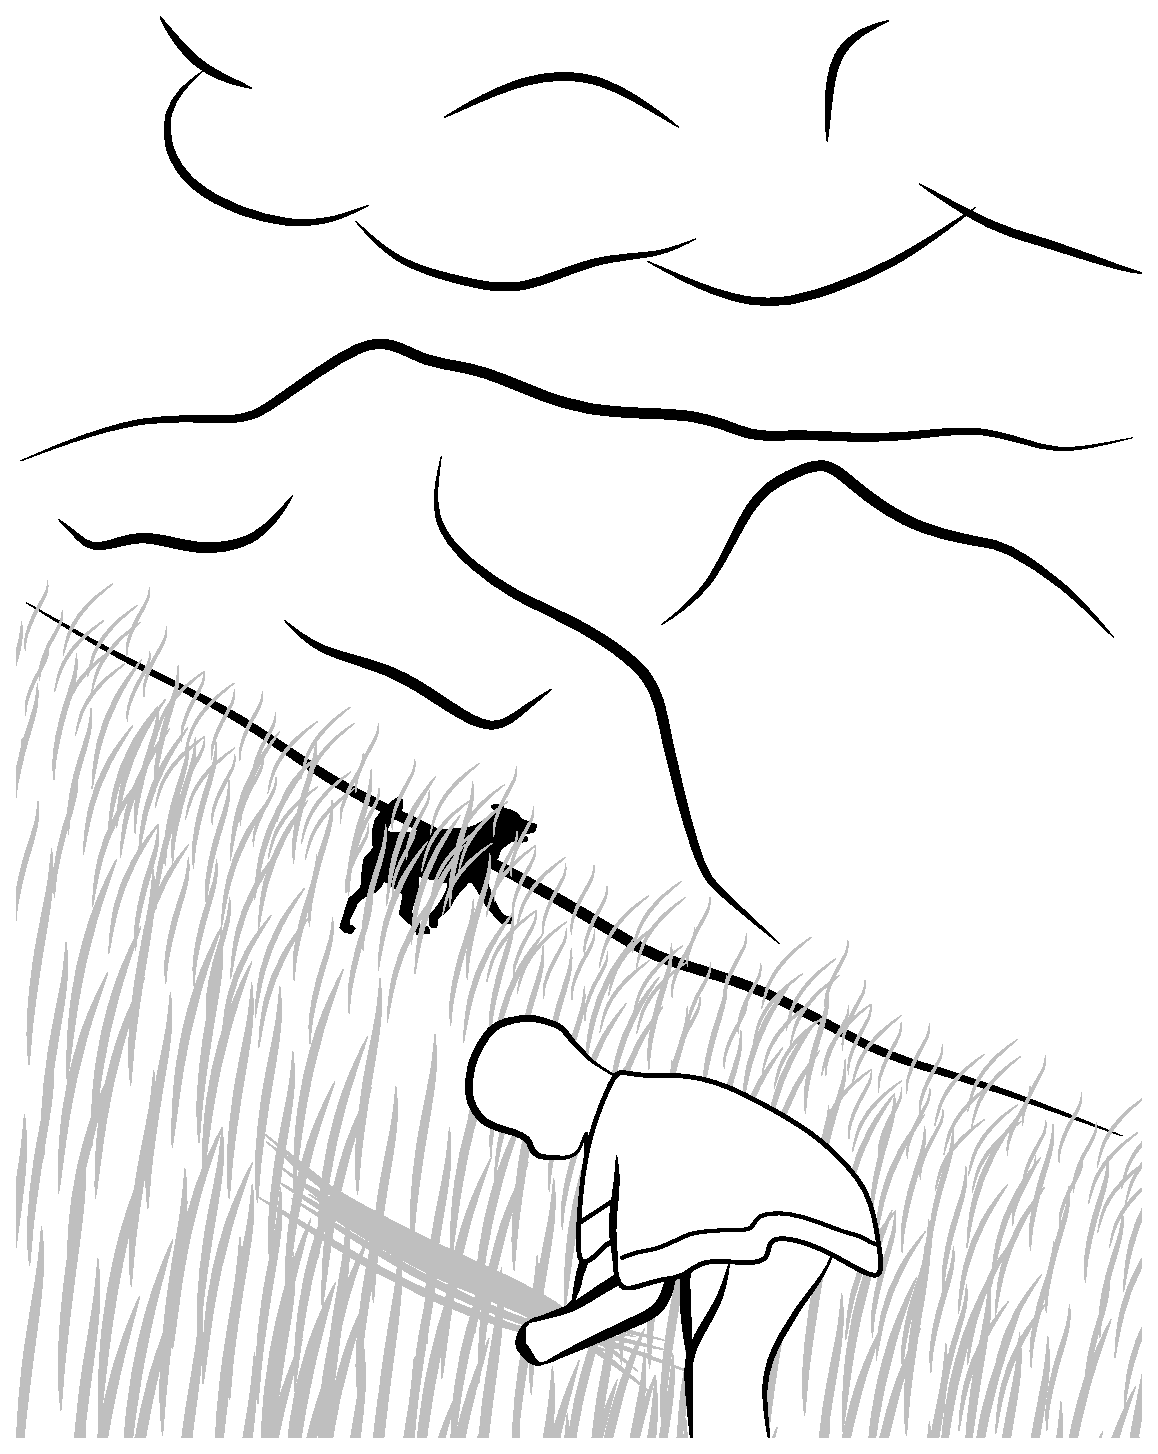
\includegraphics[width=0.43\textwidth]{pasto-zandor-aulicha}
  \end{center}
  \vspace{-20pt}
  %\caption{Figo das índias.}
\end{wrapfigure}
\fi
Desde pequeño yo llevaba a Zandor a todas mis caminatas por la sierra, como mi familia tenía vacas, yo tenía que ir a darles comida y atenderlas, y comúnmente recompensaba a Zandor por su compañía dándole leche fresca, que yo mismo ordeñaba para matar nuestra sed.
Con todos esos cuidados, en poco tiempo Zandor se volvió un cachorro fuerte y muy juguetón.
Él me ayudaba a cuidar las vacas y asustaba a los pájaros que venían a comer las semillas en la chacra. Cuando yo gritaba su nombre, él venía corriendo y se paraba frente a mí con la marcialidad de un soldado delante de su general; él era tan inteligente como una persona y mucho más obediente que yo mismo.

Un día, cuando estaba en el campo con Zandor, observamos que una perdiz salía volando de unos arbustos. Para Zandor, que aún era cachorro, fue la primera vez que él vio una perdiz; yo, por el contrario, ya tenía experiencia con esas aves y sabía que cerca a ese lugar encontraríamos un nido, huevos o crías.
Automáticamente grité:\\\indent
--- ¡Zandor! ¡Vamos a buscar huevos!\\\indent
Él ladró al sentir mi entusiasmo y avanzó junto a mí en la dirección que yo le indiqué.
Era lindo ver a Zandor, pequeño pero valiente, batiendo su cola, oliendo para todos lados, levantando y recogiendo sus orejas; como si, en aquella primera misión de búsqueda, quisiera demostrar su eficacia usando al máximo todos sus sentidos.
Solo buscamos unos minutos y de repente los vimos\\\indent
--- ¡Mira Zandor! ¡Huevos! --- grité.\\\indent
Él ladró como afirmando mi exclamación, y me acerqué al nido para recoger todos los huevos. Zandor no tomó ninguno, él solo me miraba contento en cuanto yo los colocaba en una bolsita de tela para protegerlos y llevarlos a casa.

Este procedimiento se volvió común, y cada vez que yo salía a buscar a nuestras vacas, también aprovechaba para buscar huevos de perdiz con Zandor; cuando los encontrábamos, yo los llevaba muy contento a mi mamá; de modo que, todos los días nosotros volvíamos con 8, 12 o hasta 15 huevos.
Con el pasar de los meses Zandor se volvió un especialista en encontrar huevos, además de que él ya no era un cachorro, y yo no necesitaba acompañarlo. Así, en cuanto yo trabajaba, él salía por cuenta propia a buscar huevos; en el instante que él los encontraba, ladraba para mí, varias veces y sin descanso, hasta llamar mi atención, de modo que mi única misión era recogerlos y llevarlos a casa.
\ifdefined\EnableIncludeImages
\begin{wrapfigure}{r}{0.43\textwidth}
  \begin{center}
  \vspace{-20pt}
    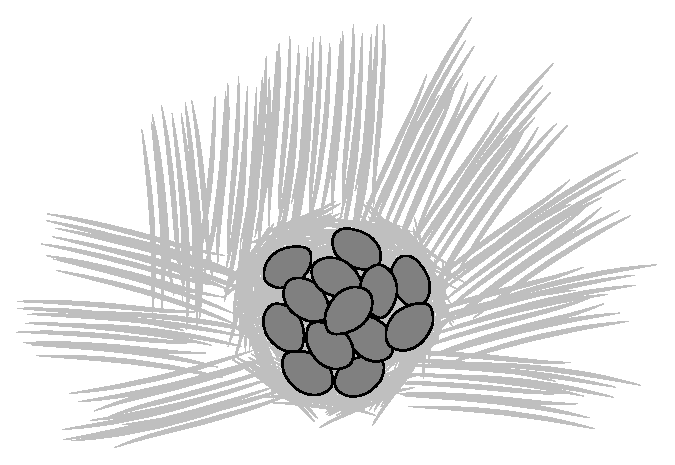
\includegraphics[width=0.40\textwidth]{huevos.eps}
  \end{center}
  \vspace{-20pt}
  %\caption{Figo das índias.}
\end{wrapfigure}
\fi
Algunas veces cocinábamos los huevos, otras veces los freíamos; siendo que en una de esas ocasiones, mi papá llegó a casa cuando estábamos cocinándolos,\\\indent
--- ¿y esos huevos?--- preguntó el, 
y nosotros contentos y llenos de orgullo respondimos:\\\indent
--- ¡Zandor los encontró!\\\indent
Él meditó un poco y replicó:\\\indent 
--- Zandor los encontró... ¿y que cosa le dieron?\\\indent 
La pregunta nos tomó por sorpresa y dijimos en voz baja:\\\indent 
--- Nada papá, solo la comida de la casa...\\\indent
Mi papá nos miró e indicó calmadamente:\\\indent 
--- Si él fue quien los encontró, él también debe participar.\\\indent
En ese momento mi papá tomó un huevo crudo y se lo dio al perro, Zandor tomó contento el huevo y lo lamió hasta dejar solamente la cáscara. A partir de entonces Zandor se acostumbró a comerlos siempre que le ofrecían. Así, cada vez que él encontraba huevos, yo los llevaba a casa, los entregaba a mi mamá y ella a su vez entregaba dos a Zandor; sin embargo, nunca le dábamos los huevos cuando él los encontraba, solamente en la casa, él por su parte sabía esperar y nunca tomó ninguno, solo esperaba pacientemente el momento que mi mamá le entregue sus huevos e iba contento a su rincón para comerlos.


Para mí Zandor era maravilloso, a cualquier lugar donde yo iba él me acompañaba, cuando estaba triste él se sentaba a mi lado y hasta lloraba conmigo haciendo un sonido agudo, que yo sentía lleno de solidaridad.
Por otro lado, si él percibía que yo estaba contento, levantaba sus orejas e iniciaba a saltar y correr de un lado a otro. Así, durante mucho tiempo, andamos y crecimos juntos... el tiempo pasó y yo cumplí ocho, y luego nueva años de edad.

Un día mi papá decidió abatir un toro; allá en la sierra no se mata a un toro sin ningún motivo, solo en ocasiones importantes como fiestas regionales, casamientos o eventos semejantes. Sin embargo, yo sabía que en esa época no teníamos ninguna festividad y pensaba que a mi papá simplemente se le había ocurrido abatir un toro sin ningún motivo, mas no era así.
Yo tenía un hermano mayor que vivía en la capital, en Lima; yo no lo conocía, solo sabia de su existencia, pues mis padres siempre hablaban sobre su vida allá y se referían a él como ``Seve'', por lo que en esa época yo pensaba que él se llamaba de esa forma, no obstante, su nombre no era ese y si Severino. Yo no lo conocía porque viajó a Lima cuando yo era muy pequeño, seguramente lo vi cuando aun era bebé, mas yo no tenia ningún recuerdo de eso.
Así, mi papá y mi mamá tenían la intención de hacer charqui para mandarlo a mi hermano como regalo, por lo que con esa finalidad decidieron abatir al toro y prepararon cuidadosamente su carne con mucha sal.

\ifdefined\EnableIncludeImages
\begin{wrapfigure}{r}{0.49\textwidth}
  \begin{center}
  \vspace{-20pt}
    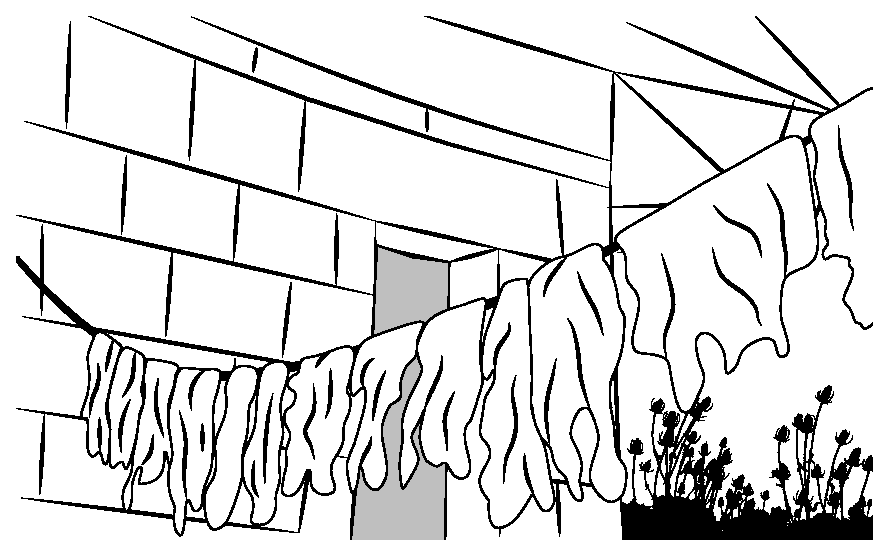
\includegraphics[width=0.47\textwidth]{charque.eps}
  \end{center}
  \vspace{-20pt}
  %\caption{Zandor}
\end{wrapfigure}
\fi
Nuestro hogar estaba compuesto por una casa pequeña y una grande, ambas separadas por varios metros entre sí; nuestra familia vivía en la casa grande y usábamos la pequeña para guardar herramientas, granos y, en general, alimentos no perecibles.
Cerca de la casa pequeña teníamos dos higueras; ese día mi papá usó una de ellas para amarrar una soga hasta la casa pequeña, y sobre ella colgó la carne para secarla con el sol, sin embargo, él decidió colgar una pierna de toro en el tronco de la otra higuera, pues esa pieza de carne pesaba mucho.
Allá la costumbre es recoger la carne y llevarla para la casa durante la noche, para que los animales de hábitos nocturnos no vengan para comerla, de modo que al día siguiente, por la mañana, con los primeros rayos de sol, la carne era nuevamente colgada; no obstante, ese día mi papá recogió solo el charqui que estaba colgado en la cuerda y se olvidó de la pierna que había colocado en la otra higuera.
Lo peor fue que allí, donde mi papá dejo la carne, tranquilamente cualquier perro, zorro, u otro animal carnívoro de la sierra, podría tomarla fácilmente, sin la necesidad de saltar, dado que no estaba a mucha altura.

Esa noche Zandor no paró de ladrar; nosotros desde la casa grande solo escuchábamos el escándalo con curiosidad, dado que ningún miembro de la familia se acordó de la pierna colgada en la higuera. Por los ruidos solo reconocíamos que algunas veces llegaban otros perros, otras veces no escuchábamos ningún otro animal, solo a Zandor ladrando con mucha rabia y fuerza; mi papá, enojado por el ruido, solo decía:\\\indent
--- ¡Que cosa quiere ese perro que no nos deja dormir!\\\indent
Sin embargo, él no salía de la casa grande a indagar sobre la situación. Yo tenía mucho miedo por todo lo que estaba sucediendo; pues, en la sierra, se cuentan historias de los seres que habitan la noche.
Algunos decían que de noche anda el ``cuco''\footnote{También llamado, coca o coco, este es un ser mítico, una especie de fantasma, bruja o espantajo que anda de noche por los caminos.}, y los niños teníamos un terror extremo a ese ser; para empeorar la situación, mi papa tenía la costumbre de contar historias sobre sus viajes, de como de noche encontró al cuco en los caminos de la sierra, o también que en algún pueblo cercano el cuco había matado a algún vecino, que había chupado la sangre de otro o simplemente asustado a algún caminante nocturno. Debo reconocer que a pesar del terror que me causaban las historias de mi papá, me gustaba conocerlas y pasar miedo escuchándolas; él siempre me contaba sus aventuras de cuando salía a trabajar a otras ciudades y las cosas que veía, los problemas que acontecían en el camino y de los personajes que aparecían cuando él se desplazaba a pié.

\ifdefined\EnableIncludeImages
\begin{wrapfigure}{r}{0.49\textwidth}
  \begin{center}
  \vspace{-20pt}
    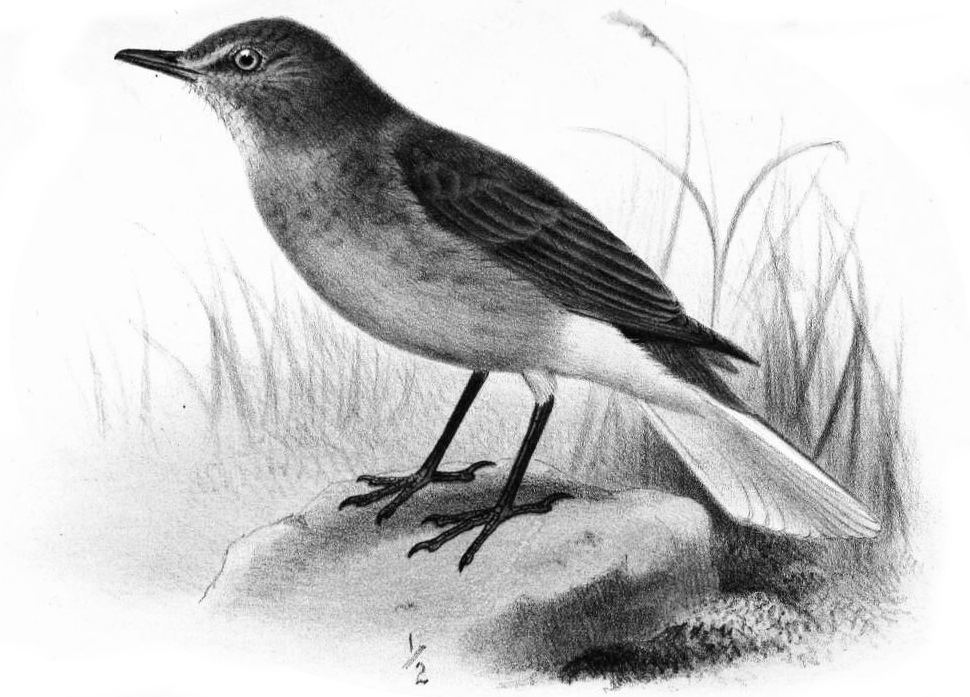
\includegraphics[width=0.47\textwidth]{AgriornisSolitariaSmit.jpg}
  \end{center}
  \vspace{-20pt}
  %\caption{Zandor}
\end{wrapfigure}
\fi
Por ejemplo, un día mi papá me contó que cuando estaba caminando viajando desde nuestro pueblo hasta ``Cangallo'', un poblado vecino, a la mitad del camino la noche lo atrapó, y empezó a buscar entre las vías una casa que pudiera darle posada. En cuanto él estaba en esa tarea, escuchó un pájaro al cual nosotros en la sierra llamamos ``huaychao''\footnote{También escrito como waychaw, esta es una palabra quechua que significa: avisar, anunciar, advertir o notificar. ``Huaychao'' es una onomatopeya del sonido que hace la ave cuyo nombre científico es Agriornis montanus.}, cuyo canto es de mal augurio.
Mi papá decía que cuando el ``Huaychao'' canta es porque el mal está cerca, que él canta porque vio al mal andando, quizás en la forma de algún ``jarjacha''\footnote{También llamado carcaq o qarqacha.}. Para nosotros los jarjachas son seres de la noche, son personas que se levantan de sus tumbas, pues al haber hecho cosas terribles en vida están condenadas a no morir y vagar de noche entre el sufrimiento y la ira.
Entonces, mi papá siempre me advertía muy serio, que si en la noche escuchaba al huaychao, debía tener mucho cuidado porque seguramente un jarjacha estaba cerca.
Siguiendo los hechos, cuando mi papá escuchó al huaychao, inició a correr saltando piedras y atravesando riachuelos hasta que, solo y asustado, encontró una casa; rápidamente tocó a la puerta y desde dentro escuchó una voz de mujer que le preguntaba:\\\indent
--- ¡Buenas noches! ¿quien anda allí?\\\indent
Mi papá todo asustado intentó explicarle que era solamente un viajero, que la noche había llegado a la mitad de su camino y que solamente necesitaba de un lugar para dormir. La señora desde el interior de la casa le respondió que, de la misma forma que él habló, seres que no son personas, cucos, andan por la noche engañando a los moradores para conseguir entrar a sus casas,\\\indent
--- ¡De repente tú eres uno de ellos! --- Indicó la señora y negó a mi papá un lugar para dormir. \\\indent
Él insistió con la voz temblorosa por el miedo, porque sabía que todo eso era verdad, pues él ya había escuchado al huaychao y sabía que el mal estaba cerca. Por fin, después de mucho insistir, la señora se conmovió y dejó a mi papá entrar a la casa.
La señora, toda curiosa por la situación, preguntó a mi papá el porqué andaba de noche, y él explicó que solo estaba intentando ir de Occo hasta Cangallo, sin embargo, tuvo problemas en el camino y la noche le ganó. Inmediatamente la señora respondió en tono maternal:\\\indent 
--- ¿Por qué andas de noche? Solo ayer un jarjacha se comió a una persona, ahora ese vecino está muerto, hoy mismo lo enterramos.\\\indent
Por todas esas historias, salir de la casa grande de noche, solo porque el perro ladraba, era una completa temeridad; hasta mi papá tenia miedo de salir, él solo gritaba para Zandor desde dentro de la casa, sujetando su ``guaraca''\footnote{Cuerda muy versátil que puede ser usada como cinturón o para disciplinar niños desobedientes.}, golpeando con ella la pared.
Los demás miembros de la familia solo escuchábamos resignados, intentando dormir a pesar del escandalo.

Así, la noche pasó, y prácticamente ninguno de nosotros consiguió dormir. Quando los primeros rayos de sol tocaron nuestra ventana, todos salimos en dirección de la casa pequeña y para nuestra sorpresa vimos la pierna de toro colgada en la higuera. Para nosotros fue evidente que durante la noche los animales del campo habían llegado a comer la carne y Zandor la había defendido, peleándose, ladrando y sin dormir. 
\ifdefined\EnableIncludeImages
\begin{wrapfigure}{r}{0.47\textwidth}
  \begin{center}
  \vspace{-0.5cm}
    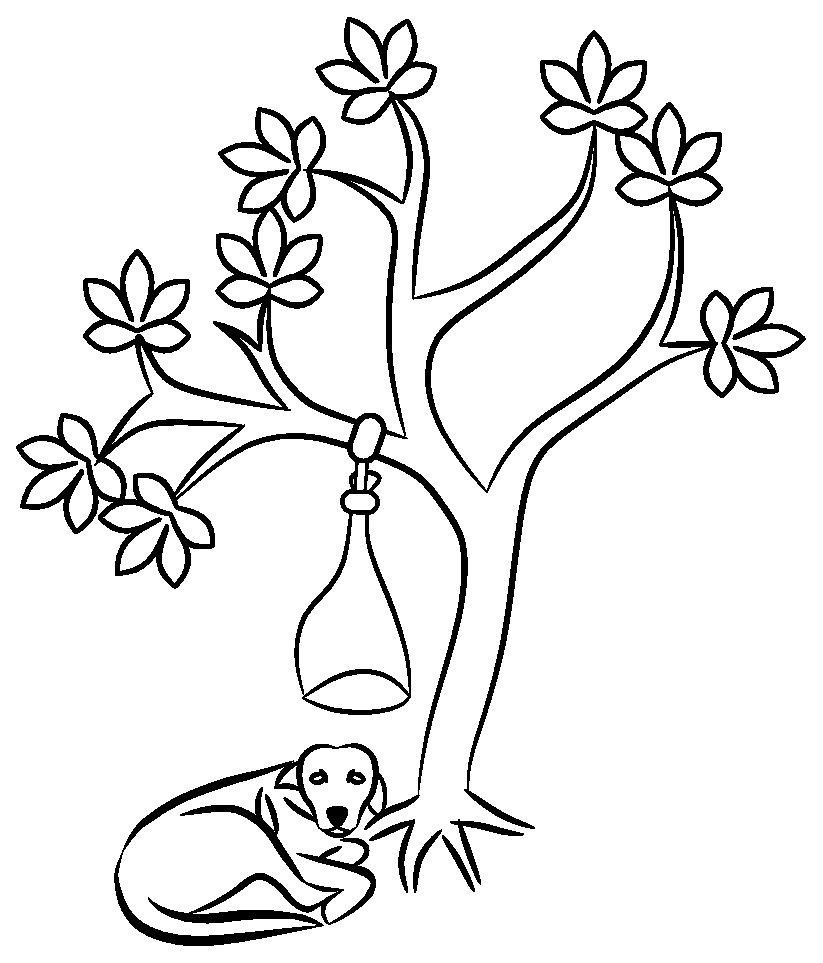
\includegraphics[width=0.45\textwidth]{perro-fiel-1.eps}
  \end{center}
  \vspace{-0.5cm}
  %\caption{Zandor}
\end{wrapfigure}
\fi
Él estaba acurrucado encogido en forma de bolita abajo de la pierna de toro y al vernos llegar solo nos dirigió una mirada cansada en cuanto batía su colita. Mi papá se admiró por el desempeño de Zandor, pues la carne estaba intacta.\\\indent
--- ¡Cómo me olvidé de la pierna! ¡Por eso llegaban los perros! exclamó mi papá.\\\indent
Automáticamente entró a la casa, tomó un cuchillo, cortó con él un pedazo grande de carne en la pierna de toro, aún colgada en la higuera, y la entregó a Zandor como un premio; solamente en ese momento él miró la carne con deseo, tomó su premio y fue para su rincón a comer.

Así, Zandor creció siendo siempre un perro honrado. Si tu no le dabas alguna cosa, él no lo tomaba, por eso toda la familia lo respetaba. Además de eso, en el campo, los perros siempre son bien cuidados; ellos comen la misma comida que los dueños de casa y son tratados con cariño, siendo ellos considerados como miembros de la familia.


